\section{Project Scope}

\subsection{Overview of the system} 
The system should allow data to be entered by medical students, junior doctors 
and  registrars  (specialists  in  training)  working  in  the  department.  People  who 
enter  data  should  have  usernames  and  passwords  (student  numbers  and 
HPCSA registration numbers can be used) and they should only be able to enter 
information  and  should  not  have  access  to  data.  They  should  be  able  to  enter 
data using smartphones, tablets or personal computers in an environment where 
the hospital is not computerized and computers are not available in the hospital 
for this purpose. \par 

For purposes  of  entering  data  smartphone and  tablet applications (apple  and 
android)  should be  developed  to  allow  smartphone  and  tablet  access  to  the 
system. \par

The data should be securely stored on a site on the Website of the University of 
Pretoria. \par

Data  will  be  entered  into  the  system  by  different  employees  working  in  the 
Department  of  Obstetrics  \&  Gynaecology  at  the  Kalafong  Provincial  Tertiary 
Hospital. \par

Data of patients entered should include both the patient’s hospital number as well 
as RSA Identity number. \par

The  possibility  of  linking  this  system  to  that  of  the  National  Health  Laboratory 
System (NHLS) should be investigated to make it possible to access laboratory 
results through this system. The NHLS has an online accessibility. \par

The  administrator  of  the  system  should  have  access  to  all  relevant  data.  The 
different levels and specifications of data output will be defined upfront and the 
ability should exist to add or edit these specifications as required. \par

Patient  information  and  data  are  highly  confidential  and  the  website  and 
information  should  be  secure.  All  users  will  have  to  use  a  username  and 
password. Medical students can use University of Pretoria student numbers and 
medical interns, medical officers and registrars can use their Health Professions 
Council  of  South  Africa  (HPCSA)  unique  registration  numbers.  Doctors  and 
students  rotate  through  the  department  for  different  time  periods  and  the 
usernames and passwords should expire depending on the different categories. 
Students  rotate  for  four  weeks,  medical  interns  for  four  months  and medical 
officers and registrars  for  up  to  five  years.  Administrative  staff  and  consultants 
are more permanent and for security reasons should perhaps update information 
yearly. \par


\subsection{Patient Information Management System - Global Scope}
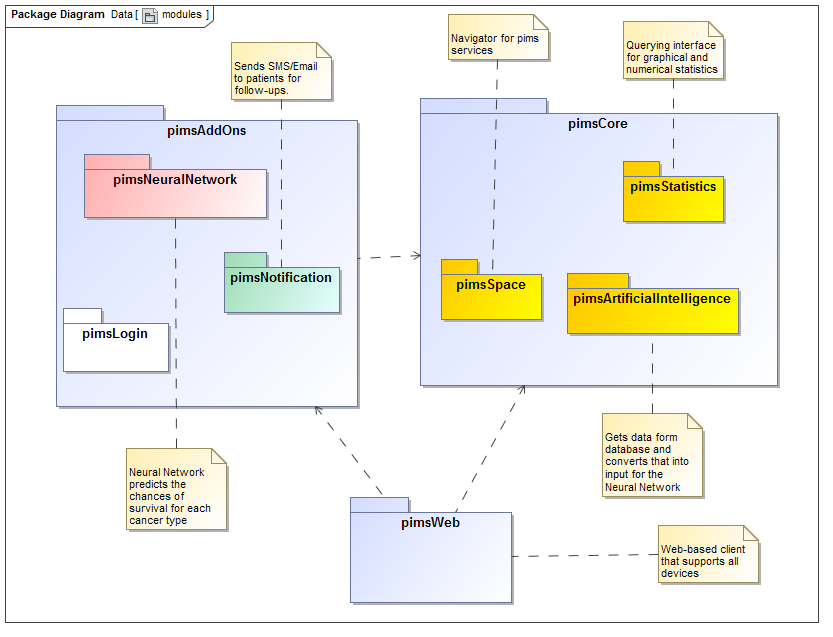
\includegraphics[width=\linewidth]{./Graphics/globalImages/modules}
